\documentclass{beamer}
\usepackage[utf8]{inputenc}
\usepackage[english,german]{babel} 
\usepackage{listings} 
\usepackage{listings-golang}
\usepackage{tikz}

\usepackage[absolute,overlay]{textpos}
  \setlength{\TPHorizModule}{1mm}
  \setlength{\TPVertModule}{1mm}

\titlegraphic{
\includegraphics[scale=0.3]{logoHaw.png}}
\title{
	\textit{BW2 Praktikum} \\
	\textbf{\\ \"Ubungsblatt 1 - Gruppe 1}
}
\author{Adrian Helberg \\ Version 1.0}
\date{\today}

\definecolor{mygreen}{rgb}{0,0.6,0}

\begin{document}
\lstset{
    frame=single,
    basicstyle=\footnotesize,
    keywordstyle=\color{blue},
    showstringspaces=false, 
    stringstyle=\color{mygreen},
    tabsize=4,
    language=Golang
}

\maketitle

\section{a)}
\begin{frame}
\frametitle{a)}

\begin{quote}
Welche Produkte und Dienstleistungen bietet Dirt Bikes an? 
\end{quote}

\begin{itemize}
\setlength{\itemsep}{20pt}
\item Motorr\"ader vom Typ ``Offroad'', eigene Marke
\begin{itemize}
\item Verschiedene Gr\"oßen, Distanzklassen
\item Enduro 250, 550
\item Moto 300, 450
\end{itemize}
\item Ersatzteil- und Servicegesch\"aft
\item Garantiereparaturen
\end{itemize}

\end{frame}

\begin{frame}
\frametitle{a)}

\begin{quote}
Wie viele Typen von Produkten und Dienstleistungen sind für die Kunden verfügbar?
\end{quote}

\begin{itemize}
\setlength{\itemsep}{12pt}
\item Motorräder, Ersatzteile als
\begin{itemize}
\item Sachgut $\rightarrow$ Konsumgut $\rightarrow$ Gebrauchsgut
\end{itemize}
\item Service, Garantie als
\begin{itemize}
\item Dienstleistung $\rightarrow$ Konsumptiv $\rightarrow$ Produktbegleitend
\end{itemize}
\end{itemize}

\end{frame}

\begin{frame}
\frametitle{a)}

\begin{quote}
Welches sind die wichtigsten Produkte für das Unternehmen?
\end{quote}

\begin{itemize}
\setlength{\itemsep}{14pt}

\item Enduro 250
\begin{itemize}
\item \$3250 St\"uckpreis $\rightarrow$ 2195x verkauft 2017
\end{itemize}

\item Enduro 550
\begin{itemize}
\item \$7600 St\"uckpreis $\rightarrow$ 3647x verkauft 2017
\end{itemize}

\item Moto 300
\begin{itemize}
\item \$4295 St\"uckpreis $\rightarrow$ 2627x verkauft 2017
\end{itemize}

\item Moto 450
\begin{itemize}
\item \$8995 St\"uckpreis $\rightarrow$ 923x verkauft 2017
\end{itemize}

\end{itemize}

\end{frame}

\section{b)}
\begin{frame}
\frametitle{b)}

\begin{quote}
Wie vertreibt das Unternehmen seine Produkte?
\end{quote}

\begin{itemize}
\setlength{\itemsep}{14pt}
\item Kein direkter Verkauf an Einzelhandelskunden
\begin{itemize}
\item Netzwerk von 40 H\"andlern
\item Unabh\"angige H\"andler f\"ur \"Ubersee (Europa)
\end{itemize}
\item Motorr\"ader, Ersatzteile und Service (einschließlich Garantiereparaturen) können nur von einem autorisierten, zertifizierten H\"andler bezogen werden
\item Bei Kunden außerhalb eines Bereichs von 50 Meilen, k\"onnen 
\begin{itemize}
\item Motorr\"ader durch einen zertifizierten, unabhängigen Motorradh\"andler gekauft werden
\item Ersatzteile direkt bei Dirt Bikes erstanden werden (Verifizierung n\"otig)
\end{itemize}
\end{itemize}

\end{frame}

\section{c)}
\begin{frame}
\frametitle{c)}

\begin{quote}
Welches sind die wert- und mengenm\"aßig wichtigsten Zulieferteile, die Dirt Bikes von Lieferanten bezieht?
\end{quote}

\begin{figure}
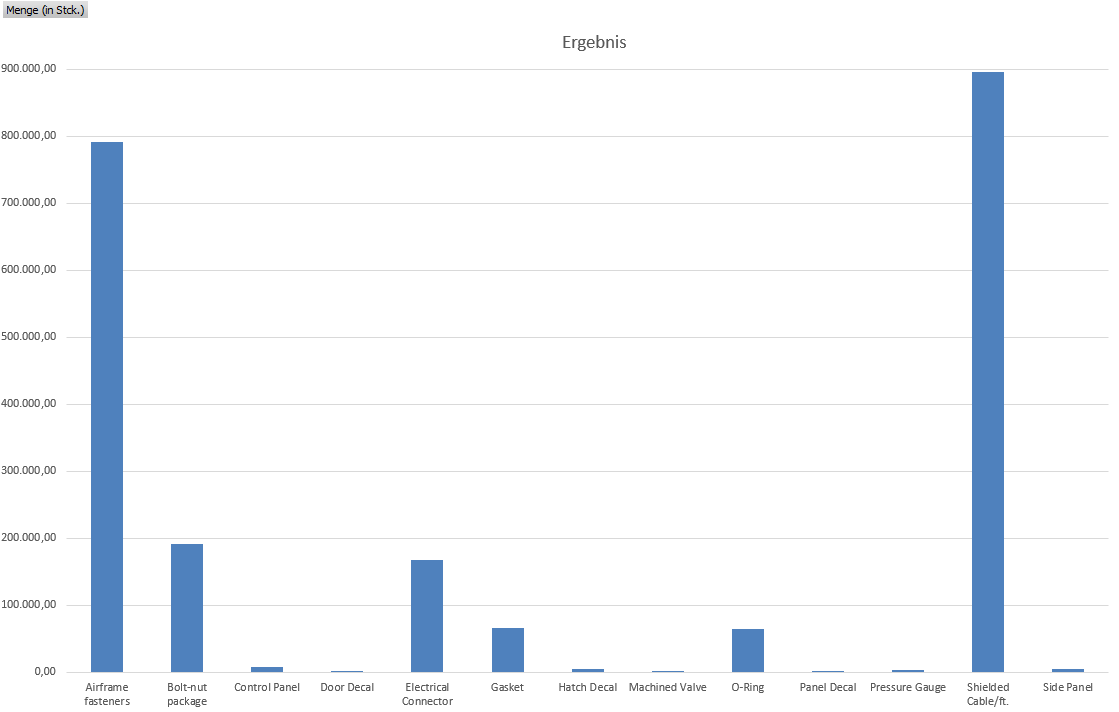
\includegraphics[scale=0.34]{pivot_itemNO_quantity.PNG}
\end{figure}

\end{frame}

\begin{frame}
\frametitle{c)}

\begin{quote}
Welches sind die wert- und mengenm\"aßig wichtigsten Zulieferteile, die Dirt Bikes von Lieferanten bezieht?
\end{quote}

\begin{figure}
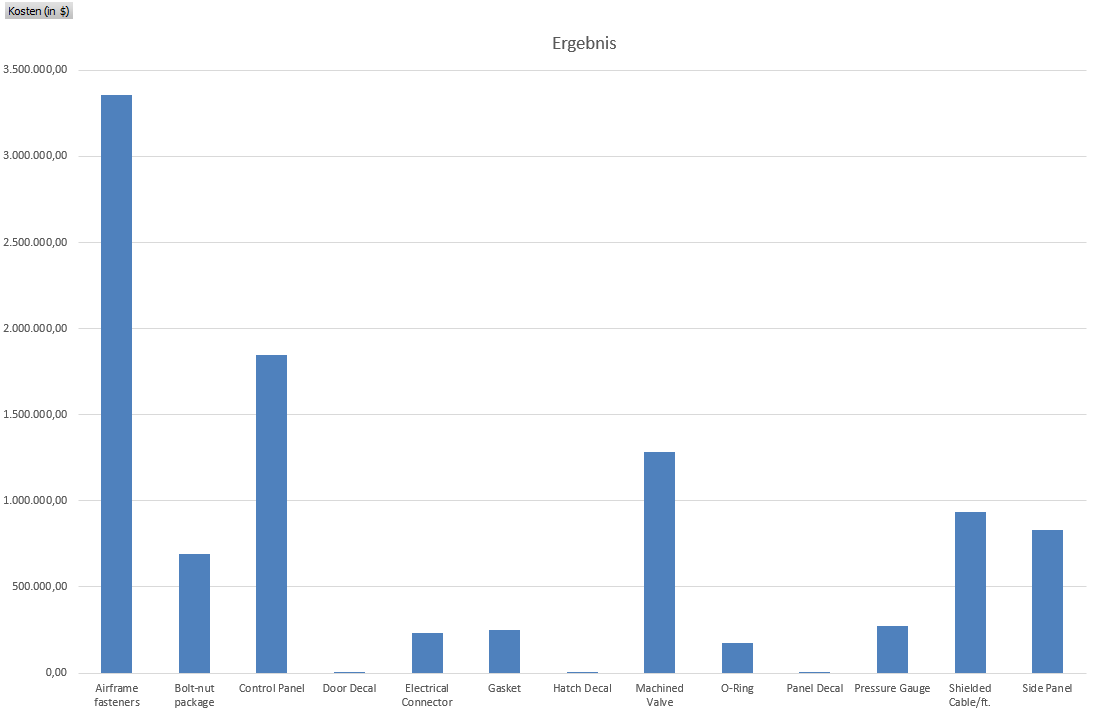
\includegraphics[scale=0.34]{pivot_itemNO_costs.PNG}
\end{figure}

\end{frame}

\begin{frame}
\frametitle{c)}

\begin{quote}
Welches sind die wert- und mengenm\"aßig wichtigsten Zulieferteile, die Dirt Bikes von Lieferanten bezieht?
\end{quote}

\begin{itemize}
\setlength{\itemsep}{14pt}
\item Mengenm\"aßig wichtigste Zulieferteile (absteigend):
\begin{itemize}
\item Airframe fasteners (Hulkey Fasteners)
\item Shielded Cable/ft.(Fast-Tie Aerospace)
\item Shielded Cable/ft.(Steelpin Inc.)
\end{itemize}
\item Wertm\"aßig wichtigste Zulieferteile: 
\begin{itemize}
\item Airframe fasteners (Hulkey Fasteners)
\item Machined Valve (Steelpin Inc.)
\item Control Panel (Alum Sheeting)
\end{itemize}
\end{itemize}

\end{frame}

\begin{frame}
\frametitle{c)}

\begin{quote}
Gibt es bei den Produkten über das Jahr auff\"allige Schwankungen? (Kosten)
\end{quote}

\begin{figure}
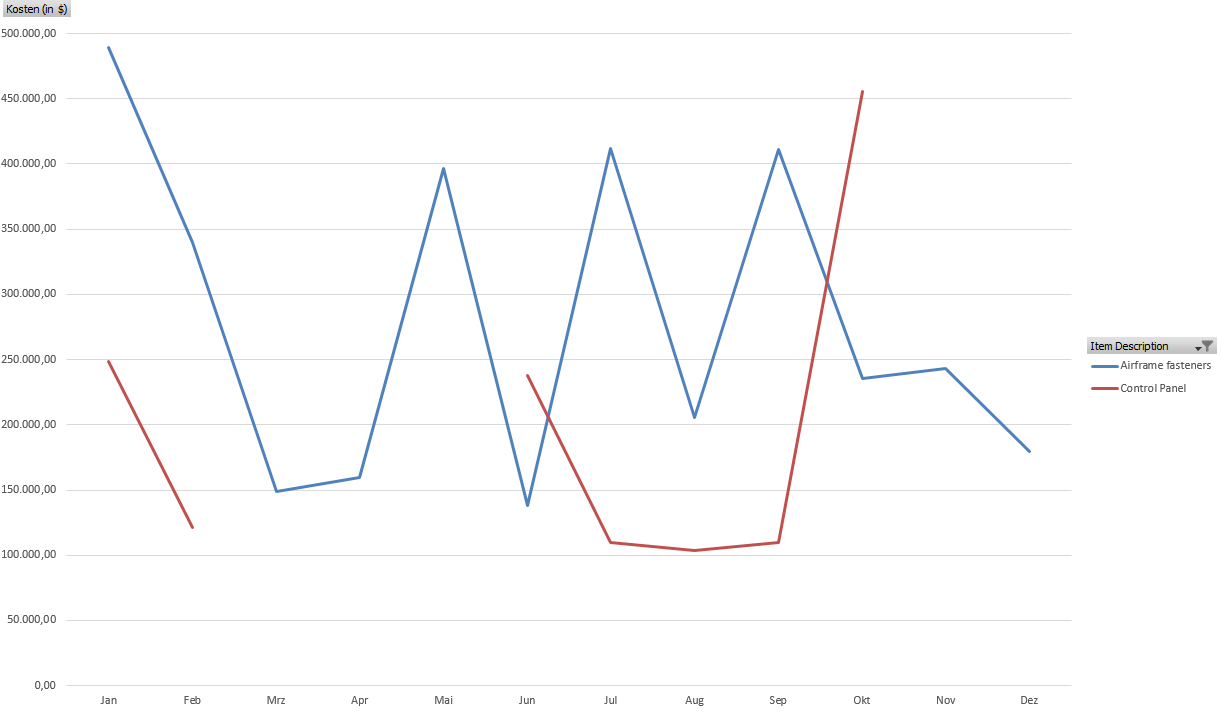
\includegraphics[scale=0.34]{pivot_itemNO_costs2.PNG}
\end{figure}

\end{frame}

\begin{frame}
\frametitle{c)}

\begin{quote}
Gibt es bei den Produkten über das Jahr auff\"allige Schwankungen? (Menge)
\end{quote}

\begin{figure}
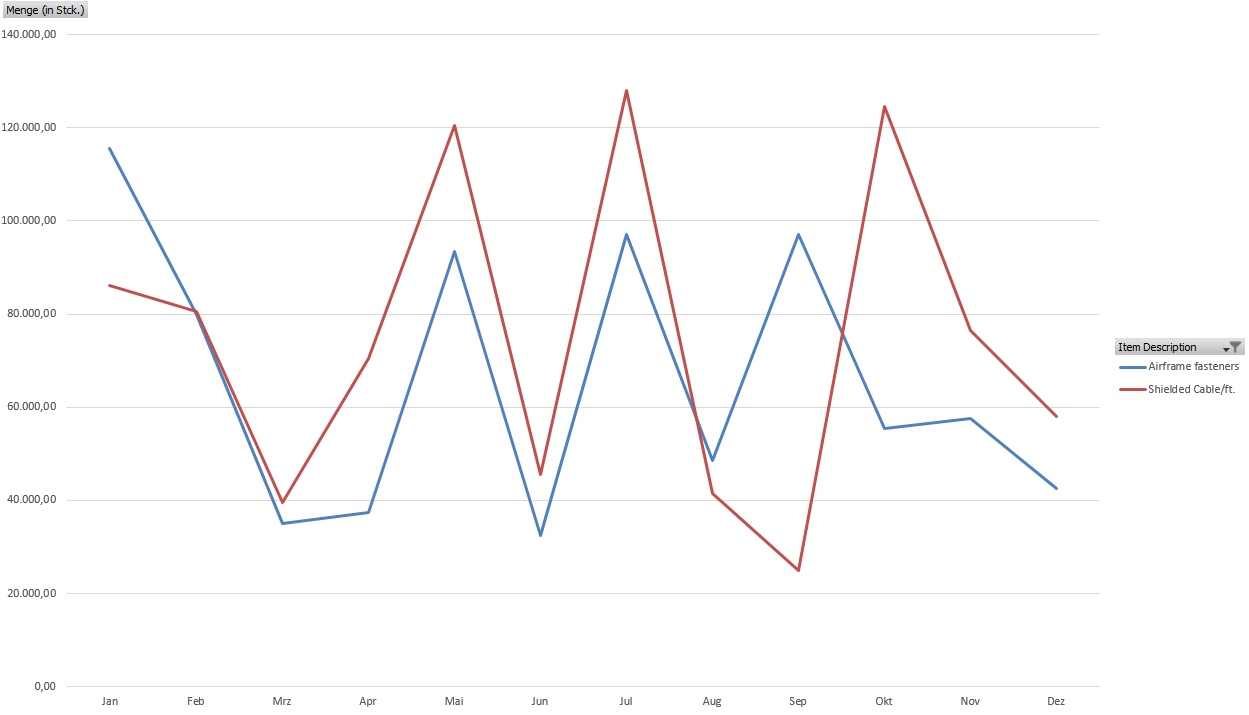
\includegraphics[scale=0.34]{pivot_itemNO_quantity2.PNG}
\caption{Bestellkosten pro Item Nummer (in \$)}
\end{figure}

\end{frame}

\begin{frame}
\frametitle{c)}

\begin{quote}
Gibt es bei den Produkten über das Jahr auff\"allige Schwankungen?
\end{quote}

\begin{itemize}
\setlength{\itemsep}{30pt}
\item Signifikante Ausschl\"age der Kosten gibt es bei den Produkten ``Airframe fasteners'' und ``Control Panel''
\item Signifikante Ausschl\"age der Menge gibt es bei den Produkten ``Airframe fasteners'' und ``Shielded Cable/ft.''
\end{itemize}

\end{frame}

\begin{frame}
\frametitle{c)}

\begin{quote}
Welches sind die wichtigsten Lieferanten für Dirt Bikes?
\end{quote}

\begin{itemize}
\setlength{\itemsep}{14pt}
\item ``Hulky Fasteners''
\begin{itemize}
\item \$3.358.200 Bestellkosten f\"ur ``Airframe fasteners''
\end{itemize}
\item ``Steelpin Inc.''
\begin{itemize}
\item 896.400 Stck. Bestellmenge f\"ur ``Shielded Cable-ft.''
\end{itemize}
\end{itemize}

\end{frame}

\section{d)}
\begin{frame}
\frametitle{d)}

\begin{quote}
Wie ist die aktuelle finanzielle Situation des Unternehmens (Aus Sicht des Jahres 2018)?
\end{quote}

\begin{figure}
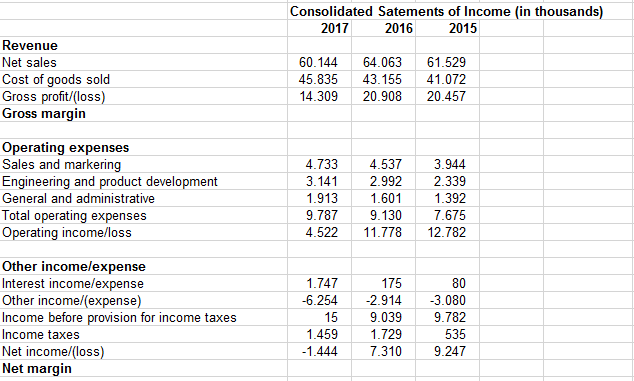
\includegraphics[scale=0.5]{financials.PNG}
\end{figure}

\end{frame}

\begin{frame}
\frametitle{d)}

\begin{quote}
\underline{Einnahmen / Ausgaben}
\end{quote}

\begin{itemize}
\item Sinkender Bruttogewinn (\$ 20.457 auf \$ 14.309)
\item Sinkende Nettoverk\"aufe (\$ 61.529 auf \$ 60.144)
\end{itemize}

$\rightarrow$ Ökonomischer Gewinn (Marge) um ca. 10\% gesunken \\ (von 33,25\% auf 23,79\%)

\end{frame}

\begin{frame}
\frametitle{d)}

\begin{quote}
\underline{Betriebsaufwand}
\end{quote}

\begin{itemize}
\item Steigender Betriebsaufwand (\$ 7.675 auf \$ 9.787)
\item Sinkendes Betriebsergebnis (\$ 12.782 auf \$ 4.522)
\end{itemize}

\begin{quote}
\underline{Sonstige Einnahmen / Ausgaben}
\end{quote}

\begin{itemize}
\item Sinkendes Nettoeinkommen (\$ 9.247 auf \$ -1.444)
\end{itemize}

\end{frame}

\begin{frame}
\frametitle{d)}

\begin{quote}
Wie ist die aktuelle finanzielle Situation des Unternehmens (Aus Sicht des Jahres 2018)?
\end{quote}

\begin{figure}
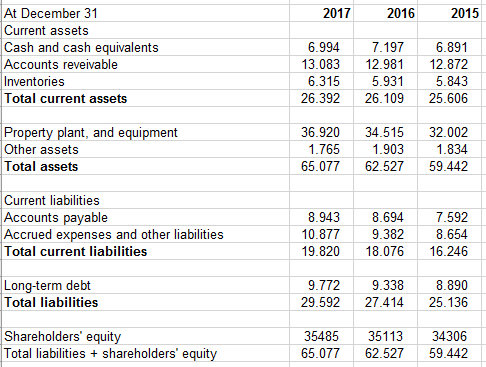
\includegraphics[scale=0.5]{financials2.PNG}
\end{figure}

\end{frame}

\begin{frame}
\frametitle{d)}

\begin{quote}
\underline{Gesamtes Umlaufverm\"ogen}
\end{quote}

\begin{itemize}
\item Steigendes Umlaufverm\"ogen (\$ 25.606 auf \$ 26.392)
\item Steigendes Gesamtverm\"ogen (\$ 59.442 auf \$ 65.077)
\end{itemize}

\begin{quote}
\underline{Verbindlichkeiten}
\end{quote}

\begin{itemize}
\item Steigende Verbindlichkeiten (\$ 16.246 auf \$ 19.820)
\item Steigende Gesamtverbindlichkeiten (\$ 25.136 auf \$ 29.592)
\item Steigende Verbindlichkeiten + Eigenkapital \\ (\$ 59.442 auf \$ 65.077)
\end{itemize}

\end{frame}

\begin{frame}
\frametitle{d)}

\begin{quote}
\underline{Warum fallen Brutto- und Netto-Gewinn?}
\end{quote}

\begin{figure}
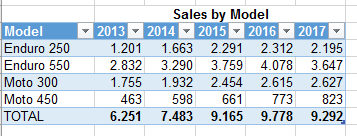
\includegraphics[scale=0.46]{financials3.PNG}
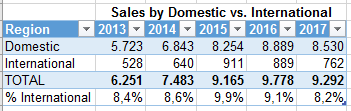
\includegraphics[scale=0.5]{financials4.PNG}
\end{figure}

\begin{itemize}
\item Sinkende Verkaufszahlen nach 2016 sowohl im inl\"andischen, als auch im internationalen Verkauf
\item Nur der Verkauf des Modells Moto 450 steigt weiterhin, was die sinkenden Zahlen der anderen Modelle aber nicht kompensieren kann
\end{itemize}

\end{frame}

\begin{frame}
\frametitle{d) - Fazit}

Dirt Bikes befindet sich in einer schlechten finanziellen Situation:
\begin{itemize}
\item Sinkender Gewinn im Kerngeschäft
\item Steigende Kosten im Betriebsaufwand
\item Sinkende Einnahmen außerhalb des Kerngesch\"afts
\item Steigenden offene, finanzielle Verpflichtungen gegenüber Gl\"aubiger
\end{itemize}

Da dennoch das Gesamtverm\"ogen steigt, bietet sich die M\"oglichkeit die finanzielle Situation zu verbessern

\end{frame}

\section{e)}
\begin{frame}
\frametitle{e)}

\begin{quote}
Welche Informationssysteme wären für ein Unternehmen wie Dirt Bikes am wichtigsten?
\end{quote}

\begin{itemize}
\item Betriebliches Informationssystem
\begin{itemize}
\setlength{\itemsep}{10pt}
\item Enterprise Architecture Frameworks (EAF)
\item Enterprise Resource Planning (ERP)
\item Supply Chain Management (SCM)
\item Customer Relationship Management (CRM)
\item E-Business-Systeme (E-Commerce)
\end{itemize}
\end{itemize}

\end{frame}

\section{a) - Teil II}
\begin{frame}
\frametitle{a) - Teil II}

\begin{quote}
Auf welche Weise k\"onnte Dirt Bikes das Internet zur Steigerung des internationalen Absatzes nutzen?
\end{quote}

\begin{itemize}
\item Das Internet k\"onnte zum elektronischen Handel (``E-Commerce'') genutzt werden
\begin{itemize}
\setlength{\itemsep}{8pt}
\item Keine Verz\"ogerung des Kaufprozesses
\item Einsicht der Produktpalette online
\item Online-Bezahlung
\item 24-Std. Service
\item Kundenn\"ahe
\item Geringe Transaktionskosten
\item Kundenkontakt auf der ganzen Welt
\end{itemize}
\end{itemize}

\end{frame}

\section{b)}
\begin{frame}
\frametitle{b)}

\begin{quote}
Mit welchen Merkmalen sollte die Website ausgestattet werden, um Käufer aus verschiedenen Zielländern anzuziehen?
\end{quote}

\begin{itemize}
\setlength{\itemsep}{6pt}
\item Website in englischer Sprache
\item Qualit\"at der Waren hervorheben
\item Sensible Daten sch\"utzen
\item Offenes Auftreten
\item Informationen \"uber das Unternehmen liefern
\item Verschiedene Landes-Dom\"anen  zur richtigen regionalen Ausrichtung
\item Internationale Kontaktm\"oglichkeiten
\item Uneingeschr\"ankte Verf\"ugbarkeit
\end{itemize}

\end{frame}

\end{document}